\documentclass[../rapport_MVEX01-11-05]{subfiles}
\begin{document}

\subsection{Färgrymder}

\begin{figure}[p]
  \centering
  \subfloat[RGB-färgrymden]{\label{fig:rgbspace-empty}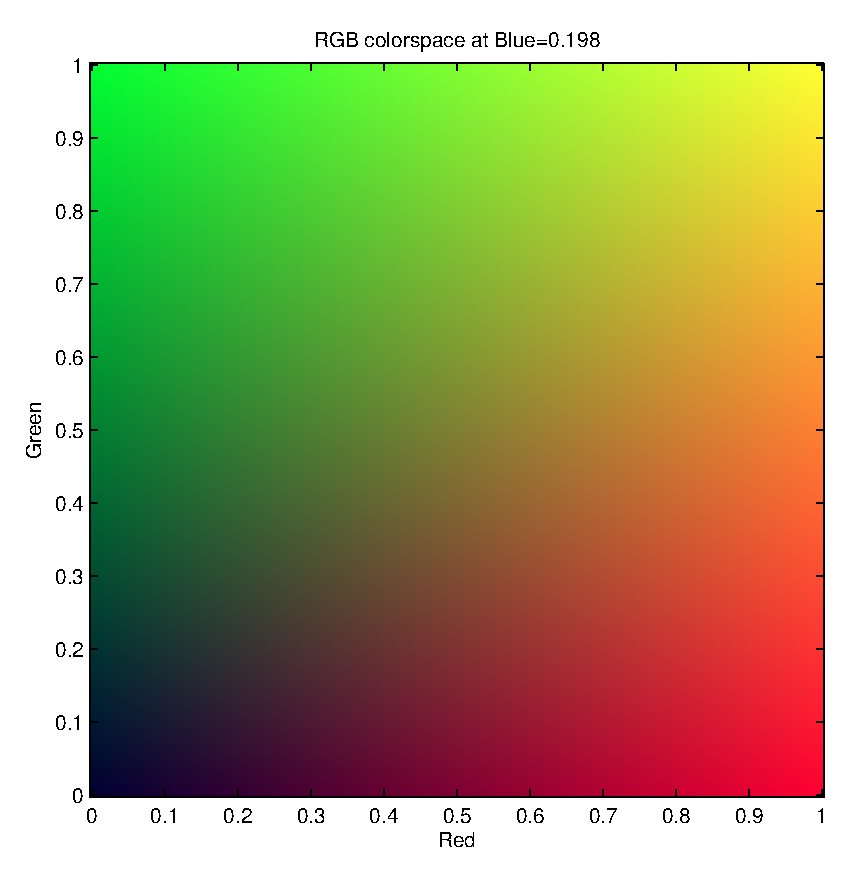
\includegraphics[width=0.45\textwidth]{bilder/colorspace}}
  \subfloat[RGB-färgrymden med ny
  basvektor]{\label{fig:rgbspace-base}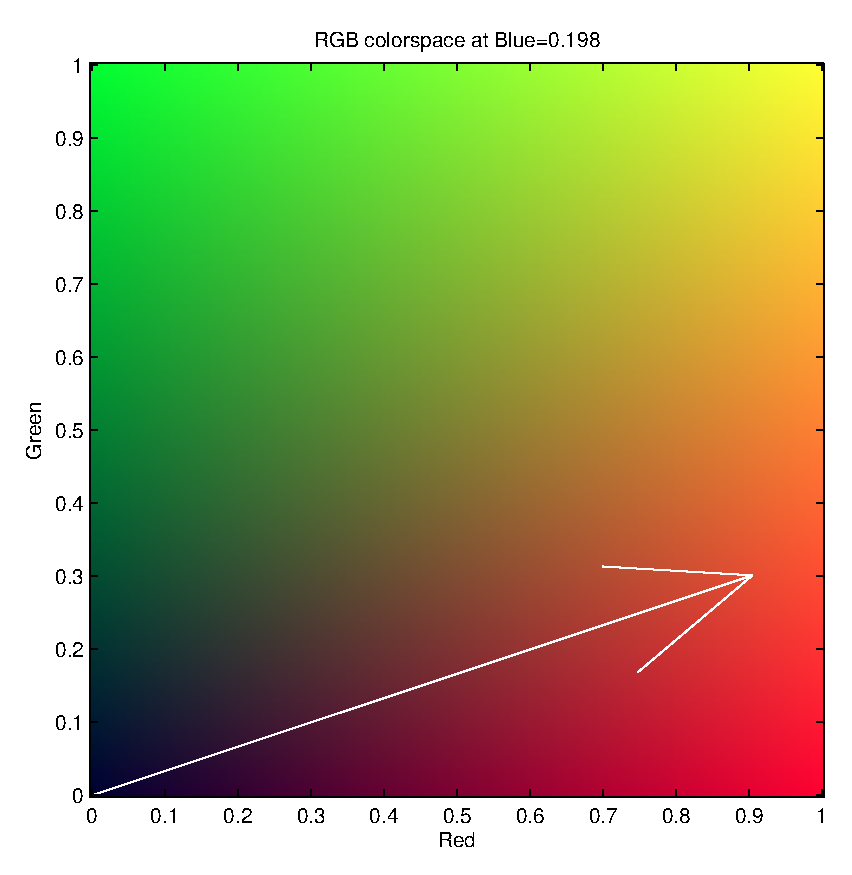
\includegraphics[width=0.45\textwidth]{bilder/colorspace_w_base}}\\
  \subfloat[RGB-färgrymden med nya
  basvektorer]{\label{fig:rgbspace-bchange}\includegraphics[width=0.7\textwidth]{bilder/colorspace_base_changed}}\\
  \caption{Processen för att ta fram en ny bas i färgrymden består av tre steg.}
  \label{fig:rgbspace}
\end{figure}

\end{document} 